\noindent
\begin{tabular}{cc}
\begin{minipage}[]{0.60\textwidth}
%\sectionIf{\flagSect}{\taitol{Esercizio}}
%\vspace{-2.5cm}
\begin{exercise}[Manometro e Venturi]
Si consideri il manometro riportato in figura utilizzato per misurare la
differenza di pressione esistente fra due sezioni diverse di un condotto.
Determinare la differenza di pressione fra i punti $A$ e $B$ riportati
sul disegno sapendo che il liquido manometrico \`e acqua e ha
una densit\`a di $998\ kg/m^3$, che il fluido che scorre all'interno 
del condotto \`e aria e ha una densit\`a di $1.225\ kg/m^3$,
che $h_A = 1\ m$, che $h_B = 1.2\ m$, che $h_0= 0.1\ m$,
che $h_1 = 0.3\ m$ e che $h_2 = 0.7\ m$.\\ 
($p_B-p_A=-3913.75\ Pa$)
\end{exercise}
\end{minipage}%
&
\begin{minipage}[ ]{0.30\textwidth}
   {}
   \begin{center}
   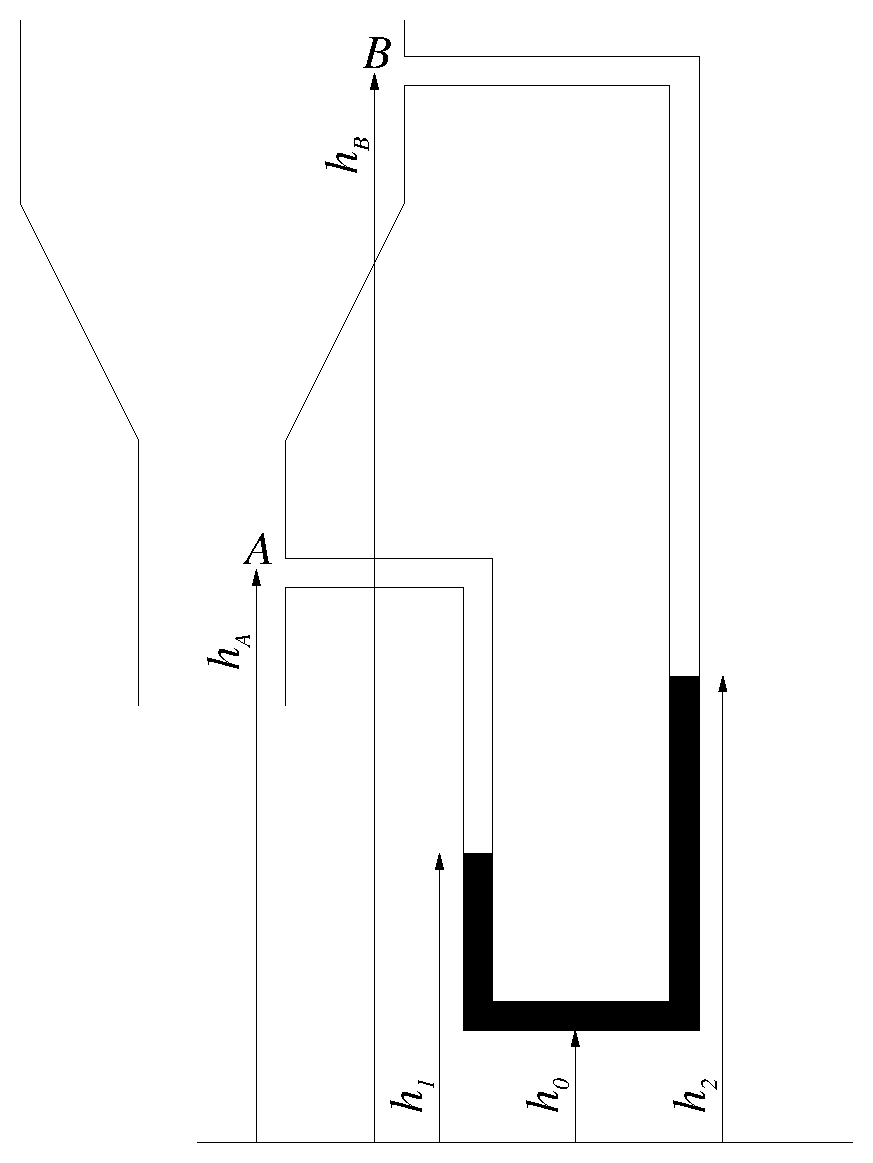
\includegraphics[width=0.90\textwidth]{./fig/manometro.eps}
   \end{center}
\end{minipage}
\end{tabular}

\sol

\partone Legge di Stevino. Manometro. Venturi.
%
\begin{equation}
   P_1 + \rho g h_1 = P_2 + \rho g h_2
\end{equation}

\parttwo
 Si scrive la legge di Stevino tra i punti A e 1, 1 e 2, 2 e B:
\begin{equation}\label{eqn:stevino:underdet}
\begin{cases}
  P_B + \rho_a g z_B = P_2 + \rho_a g z_2  \\
  P_1 + \rho g z_1 = P_2 + \rho g z_2   \\
  P_A + \rho_a g z_A = P_1 + \rho_a g z_1 \\
  \Delta P = P_B - P_A 
\end{cases}
\end{equation}
Si risolve il sistema lineare (come più piace). Ad esempio, partendo dalla terza e inserendo nella seconda e nella prima i risultati trovati:
\begin{equation}
\begin{aligned}
 & P_1 = P_A + \rho_a g (z_A - z_1) \\
 & P_2 = P_A + \rho_a g (z_A - z_1) + \rho g (z_1 - z_2) \\
 & P_B = P_A + \rho_a g (z_A - z_1) + \rho g (z_1 - z_2) + \rho_a g (z_2 - z_B)
\end{aligned}
\end{equation}
E quindi, portando $P_A$ a sinistra:
\begin{equation}
  \Delta P = -(\rho - \rho_a) g ( z_2-z_1) - \rho_a g (z_B - z_A) = -3909.8 Pa
\end{equation}

\paragraph{Osservazione.} Il sistema lineare (\ref{eqn:stevino:underdet}) è sotto determinato (se esiste una soluzione, ne esistono infinite), essendo un sistema lineare di 4 equazioni in 5 incognite, $P_1$, $P_2$, $P_A$, $P_B$, $\Delta P$. Il sistema lineare può essere scritto usando il formalismo matriciale come $\underline{\underline{A}}\,\underline{x} = \underline{b}$ con
\begin{equation}
 \underline{\underline{A}} = 
\begin{bmatrix}
  0 &  1 &  0 & -1 &  0 \\
  0 &  0 & -1 &  1 &  0 \\
 -1 &  1 &  1 &  0 &  0 \\
  1 & -1 &  1 &  0 &  0 \\
\end{bmatrix} , \quad
 \underline{x} = \begin{bmatrix}
  P_A \\ P_B \\ P_1 \\ P_2 \\ \Delta P
\end{bmatrix} , \quad
 \underline{b} = \begin{bmatrix}
  \rho_a g (h_2-h_B) \\ \rho g (h_1-h_2) \\ \rho_a g (h_A-h_1) \\ 0 
\end{bmatrix} \ .
\end{equation}
Poichè la matrice $\underline{\underline{A}}$ ha rango massimo (=\,4), esiste una soluzione $\underline{x}^*$ del problema, tale che  $\underline{\underline{A}}\,\underline{x}^* = \underline{b}$. Dal teorema del rango, si sa che il numero delle colonne (=\,5) di una matrice è uguale alla dimensione del suo rango (=\,4) e del suo nucleo (quindi =\,1). Il nucleo della matrice $\underline{\underline{A}}$, tutti i vettori $\underline{v}$ t.c.  $\underline{\underline{A}}\,\underline{v} = \underline{0}$, è uno spazio vettoriale di dimensione uno.
Se $\underline{x}^*$ è soluzione del sistema, allora anche tutti i vettori $\underline{x}^* + a \underline{v}$, $a \in \mathbb{R}$, sono soluzione del sistema, poichè $\underline{\underline{A}}(\underline{x}^* + \underline{v}) = \underline{\underline{A}}\,\underline{x}^* + \underline{\underline{A}}\,\underline{v} = \underline{b} + \underline{0}$.
 Si può dimostrare il nucleo di $\underline{\underline{A}}$ è generato dal vettore $\underline{v}=(1,1,1,1,0)^T$. Quindi le infinite soluzioni del problema hanno la forma
\begin{equation}
 \begin{bmatrix}
  P_A \\ P_B \\ P_1 \\ P_2 \\ \Delta P 
 \end{bmatrix} = 
 \begin{bmatrix}
  P_A^* \\ P_B^* \\ P_1^* \\ P_2^* \\ \Delta P 
 \end{bmatrix} + 
 \begin{bmatrix}
   a \\ a \\ a \\ a \\ 0
 \end{bmatrix} \ .
\end{equation}
Ora dovrebbe apparire chiaro come non sia possibile determinare il valore assoluto delle pressioni $P_1$, $P_2$, $P_A$, $P_B$ solamente da una misura di pressione con un manometro \textit{differenziale}: questi valori sono noti a meno di una costante additiva $a$, indeterminata. Al contrario, la differenza di due di questi valori, come $\Delta P = P_B - P_A$, è unica (e uguale al risultato ottenuto nello svolgimento del problema): l'unicità di $\Delta P$ dipende dalla forma dei vettori del nucleo di $\underline{\underline{A}}$ che hanno componente $\Delta P$ nulla.



 
